\documentclass{article}
\usepackage{arxiv}

\usepackage[utf8]{inputenc}
\usepackage[english, russian]{babel}
\usepackage[T1]{fontenc}
\usepackage{url}
\usepackage{booktabs}
\usepackage{amsfonts}
\usepackage{nicefrac}
\usepackage{microtype}
\usepackage{lipsum}
\usepackage{graphicx}
\usepackage{svg}
\usepackage{graphicx}
\usepackage{subcaption}
\usepackage{natbib}
\usepackage{doi}
\usepackage{booktabs}
\usepackage{float}
\usepackage{mathtools}
\usepackage[russian]{babel}      % пакет русификации
\usepackage{amsmath}
\usepackage{tikz}                % для создания иллюстраций
\usepackage{pgfplots}            % для вывода графиков функций
\usepackage{geometry}		 % для настройки размера полей
\usepackage{hhline}
\usepackage{placeins}
\usepackage{indentfirst} 
\usepackage{placeins}
% для отступа в первом абзаце секции
\usepackage{multirow}            % для таблицы с результатами
\usepackage{svg}
\usepackage{makecell}
\usepackage{listings}
\usepackage{float}
\usepackage[unicode, colorlinks, linkcolor=Black]{hyperref}

\title{Нейросетевой подход к обучению векторных представлений мультимодальных данных на основе угловых аддитивных функций потерь}

\author{ Черникова Полина Георгиевна \\
	ВМК МГУ\\
	\texttt{p.chernikova@yandex.ru} \\
	%% examples of more authors
	\And
	Воронцов Константин Вячеславович \\
	ВМК МГУ\\
	\texttt{vokov@forecsys.ru} \\
}
\date{2023}

\renewcommand{\shorttitle}{Обучение векторных предаставлений мультимодальных данныхина основе угловых аддитивных функций потерь}

%%% Add PDF metadata to help others organize their library
%%% Once the PDF is generated, you can check the metadata with
%%% $ pdfinfo template.pdf
\hypersetup{
pdftitle={Обучение векторных представлений мультимодальных данных},
pdfsubject={q-bio.NC, q-bio.QM},
pdfauthor={Черникова П.Г., Воронцов К.В.},
pdfkeywords={First keyword, Second keyword, More},
}

\begin{document}
\maketitle
\begin{abstract}
В данной работе рассматривается задача обучения метрического представления мультимодальных данных. Для ее решения предлагается новый подход обучения с учителем на основе сферического классификатора и аддитивных угловых функций потерь.  
Предлагаемый подход состоит из двух основных компонентов: 1) двухуровневой архитектуры на базе трансформеров; 2) аддитивной угловой функции потерь, напрямую оптимизирующей сферическое расстояние между объектами.
Эксперименты показали, что данный подход позволяет ускорить обучение, получить более разделимые и геометрически интерпретируемые векторные представления по сравнению с классическими подходами.
Предложенная архитектура легковесна, эффективно скалируется при увеличении количества данных и модальностей, не требуя перебора комбинаторного числа пар, как контрастивное обучение. 
\end{abstract}


\keywords{Векторное представление \and Мультимодальные данные \and Аддитивная угловая функция потерь \and Нейронные сети}

\section{Введение}
\par Задача обучения векторных представлений - это задача машинного обучения, в ходе которого алгоритмы извлекают значимые закономерности из исходных данных и создают представления, которые легче понять и обработать. Выученные пердставления используются для широкого класса задач, таких как: поиск, рекомендации, кластеризация, классификация и т.д. \cite{9068414}.

Важной частью данной задачи является обучение на мультимодальных данных, то есть данных из разных источников, разной природы \cite{ngiam2011multimodal}. В реальном мире большинство задач основаны на мультимодальных данных: рекомендации в e-commerce \cite{Bai_2023_ICCV}, медицине \cite{huang2021gloria}, робототехника \cite{9354900} и т.д.  Кроме того, добавление мультимодальных данных может значительно учлушить результаты решаемой задачи \cite{8949228}. 

При построении векторных представлений мультимодальных данных основной трудностью и темой для исследований является задача смешения (фьюжена) данных - интеграция информации, извлеченной из каждой модальности в единое компактное представление. Методы фьюжена можно разделить в зависимости от стадии, на которой происходит слияние данных, на ранние и поздние. При раннем фьюжене данные соединяют до применения к ним модели, при позднем - данные каждой модальности подаются на вход соответсвующим моделям, и уже их выходные признаковые представления конкатенируются. Последние исследования \citep{zhang2020multimodal} используют промежуточный фьюжен, когда слияние происходит на нескольких слоях глубокой сети. Промежуточный фьюжен может быть реализован 
\begin{itemize}
    \item \textbf{простыми операциями} конкатенирования, взвешенных сумм (полносвязный слой) или их суперпозиции \cite{nikzad2021berters};
    \item с помощью \textbf{механизмов внимания}, которые зачастую представляют из себя взвешенную суму набора векторов с весами, которые генерируются динамически на каждом шаге маленькими моделями; 
    \item с помощью билинейного пулинга, который создает совместное представление для векторов двух модальностей, вычисляя их внешнее произведение
\end{itemize}
  
Существует 3 основных нейросетевых фреймфорка для построения мультимодальных векторных представлений \citep{8715409}:
\begin{itemize}
    \item совместное представление (joint representation), выучивающее общее семантическое пространство для всех модальностей
    \item координированное представление (coordinated representation), выучивающее отдельные представления для каждой модальности, которые координированы за счет ограничений (констрейнов)
    \item система энкодер-декодер, которая переводит одну модальность в другую, сохраняя их семантику согласованной
\end{itemize}

\par Большинство современных нейросетевых методов обучения векторных представлений мультимодальных данных для доменных задач поиска и рекомендаций сегодня реализованы на основе фреймворка joint representation и используют контрастивное обучение \cite{Bai_2023_ICCV}, \cite{Dong_2022_CVPR}, \cite{huang2019multimodal}. Этот подход показывает результаты, сравнимые с SOTA, однако имеет ряд недостатков. Так для контрастивного обучения требуется подготовка большого количества положительных и отрицательных пар объектов, которое возрастает комбинаторно с ростом размера датасета, что приводит к долгому и ресурсозатратному обучению. 
В основном в качестве модальностей используется пара: изображение - текст, при этом игнорируется важность дополнительной информации из табличных данных, категориальных признаков и взаимосвязей. Однако, как показано во множестве работ \cite{}. 

\par В данной работе предлагается новый подход обучения метрических векторных представлений мультимодальных данных, использующий совместное представление модальностей на сфере и угловех аддитивные функций потерь. Похожий подход на основе сферического классификатора и угловых аддитивных функций потерь зарекомендовал себя в задаче распознания лиц \cite{deng2019arcface}. Он не только ускорил обучение на больших датасетах, но и повысил дискриминативную способность векторных представлений признаков в сравнении с контрастивным обучением. Предложенный  фреймворк состоит из двух основных компонентов: двухуровневой архитектуры на базе трансформеров и аддитивной угловой функции потерь, напрямую оптимизирующей сферическое расстояние между объектами. Этот фреймворк позволяет  эффективно увеличивать количество данных и модальностей, не требует перебора комбинаторного числа пар, как контрастивное обучение, и обучает компактные, разделимые векторные представленяи, которые хорошо подходят для задач поиска, кластеризации и рекомендаций.



\section{Задача обучения метрических векторных представлений на мультимодальных данных}
Цель обучения метрических векторных представлений мультимодальных данных состоит в том, чтобы выучить общее пространство представлений, которое отражает признаки каждой модальности и внутрениие взаимосвязи между ними. Полученные в этом пространстве представления разделимы и репрезентативны. Представления похожих объектов, то есть объектов относящихся к одной гипотетической категории должны быть близки. 
Формализуем данную постановку.
Пусть у нас есть набор данных $D$ c модальностями $М$, где $|M| = n$.

Пусть $d_i \in D$ - набор данных из $n$ модальностей, описывающий $i$-й объект, где $i \in \hat{1,n}$;
$Y$ - множество множество гипотетических категориий. В общем случае это множество не ограничено. Каждой категории может принадлежать сразу несколько наборов данных $d_i$.
Надо найти такое отображение $f: D \rightarrow R$, что:


$$\underset{i=j}{\text{sim}}(r_{y_i}, r_{y_j}) < \underset{i \neq j}{\text{sim}}(r_{y_i}, r_{y_j}) \forall i,j \in \mathbf{N}, r \in R$$

где: 
\begin{itemize}
    \item $r_{y_i}$ - вектор из R, принадлежащий категории $y_i$
    \item ${\text{sim}}(A, B) = \frac{A*B}{||A||*||B||}$ - косинусная близость векторов
\end{itemize}

Конкретно в нашей задаче будем использовать следующие n = 3 модальности:
\begin{enumerate}
    \item $T$ - текст
    \item $C$ - категориальные
    \item $V$ - табличные данные
\end{enumerate}
Так как у нас нет информации о количестве всех классов (категорий), будем использовать прокси метрику ROC-AUC на бинарной клссификации принадлежности пары к одному классу. В качестве уверенности модели будем использовать косинусную близость между объектами пары. 
$$\text{ROC-AUC} = 1 - \int_{0}^{1} \text{FRR} \, d\text{FAR}$$, где 

$\text{FRR} = \frac{\text{False Negatives}}{\text{False Negatives} + \text{True Positives}}$


$\text{FAR} = \frac{\text{False Positives}}{\text{False Positives} + \text{True Negatives}}$

\section{Решение}

\subsection{Архитектура}
\begin{figure}[H]
  \centering
  \includegraphics[width=1\linewidth]{framework.png}
  \caption{Модель на вход принимает данные трех модальностей: текст, табличные данные, категориальные признаки. Каждая модальность представляется вектором признаков, полученным с помощью трансформера, специфичного для этой модальности. Полученные вектора конкатенируются и подются на вход смешивающей сети. Смешивающая сеть обучается с помощью сферической головы ArcFace и кросс-энтропии. На этапе инференса полученные в смешивающей сети компактный и дискриминативные представления можно использовать в задачах мултимодального поиска, кластеризации, классификации и построения рекомендаций.}
  \label{fig:fig1}
\end{figure}
В качестве решения предлагается фреймворк, архитектура которого представлена на рис. \ref{fig:fig1}.
Для каждой модальности данных используется свой модально-специфичный трансформер. Так для текста на английском языке мы использовали Sentence BERT \cite{reimers-2019-sentence-bert}. Для табличных и каткгориальных данных могут быть использованы предобученные трансформерные модели для структурированных и текстовых данных на основе BERT, например, TaBERT \cite{yin2020tabert} или Tabbie \cite{iida2021tabbie}. Однако в данном случае мы использовали простейшее кодирование признаков: нормализацию вещественных признаков и one-hot encoding для категориальных. Полученные векторные представления конкатенируются и подаются на вход смешивающей нейронной сети (Fusion network), которая в базовом виде состоит из одного полносвязного слоя, проектирующего мультимодальный вектор в общее пространство признаков. Смешивающая сеть обучается с помощью головы сферического классификатора ArcFace \cite{deng2019arcface} и кросс-энтропии. Идея состоит в том, чтобы отобразить представление на гиперсферу и с помощью аддитивной угловой функции потерь (additive angular margin loss) раздвинуть векторы признаков, принадлежащие разным классам.

\par Формально сферическая классификационная голова работает следующим образом:
\begin{itemize}
    \item Пусть на выходе полносвязного слоя смешивающей сети мы получили вектор $x \in \mathbf{R}^d$. Нормализуем его, чтобы отобразить на сферу: $||x||_2 = 1$
    \item Нормализованный вектор может быть представлен следующим образом: $$\frac{W^Tx}{||W^Tx||_2}$$, где $W \in \mathbf{R}^{d \times n}$ - матрица весов полносвязного слоя, $n$ - число классов (число категорий в нашей постановке), $x$ - сконкатенированный модальности вектор, который мы подаем на вход полносвязному слою нашей смешивающей сети. 
    \item Логиты сети для класса $y_i$ могут быть получены как  скалярное произведение матрицы весов на вектор признаков, полученных на выходе полносвязного слоя: $W_{y_i}^Tf = ||W_{y_i}||||f||\cos\theta_i$, где $W_{y_i}$ - $i$-й столбец матрицы W, соответсвующий классу $y_i$, $\theta_i$ - угол между весом $W_{y_i}$ и признаков $f_i$.
    \item С помощью l-2 нормализации, аналогично $x$, приведем $||W_i||=1$, а $||W_i||=1$ скалируем до длины радиуса гиперсферы $s$, на которую отображаем признаки. Такая нормализация признаков и весов приводит к тому, что теперь предсказания зависят только от угла между признаками и весами. 
    \item Таким образом выученные векторные представления признаков распределены на гиперсфере радиуса $s$.
    \item Чтобы раздвинуть признаки, принадлежащие разным классам, введем штрафную добавку $m$ между $x_i$ и $W_{y_i}$. Таким образом получим аддитивную угловую функцию потерь, штрафующую геодезическое расстояние между классами:
    $$L = \log\left(\frac{e^{s(\theta_{y_i} + m)}}{e^{s(\theta_{y_i} + m)} + \sum_{j \neq y_i} e^{s \theta_j}}\right)$$
где 
\begin{itemize}
  \item \(s\) радиус гиперсферы или скалирующий коэффициент,
  \item \(\theta_i\) - векторное представление $i$-го признака в углвой форме
  \item \(y_i\) - реальныя метка класса (категории) \(i\)-го вектора признаков.
  \item \(m\) - угловая добавка
\end{itemize}

\end{itemize}

В геометрической интерпретации сефрическая классификационная голова отображает вектора признаков на сферу таким образом, чтобы признаки одного класса концентрировались на сфере под одним углом. Аддитивная угловая функция потерь с помощью углового сдвига раздвигает признаки от границы решений (decision boundery), тем самым обучает разделимые векторные представления. 

\par Предложенная архитектура легковесна.

\subsection{Данные}
Для проведения экспериментов и тестирования модели, предложенной в качестве решения, был взят набор Google Local Reviews картах 2021, содержащий информацию о компаниях и отзывах о них на Google картах. Этот датасет использовался в похожих работах про мультимодальность и контрастивное обучение \cite{li2022uctopic}, \cite{yan2023personalized}.
\par  В качестве датасета для теста была выбрана часть исходного датасета - метаданные о всех компаниях в Калифорнии. Эти данные содержали информацию о 515,961 компаниях. Набор данных о компании содержал признаки 3 модальностей (см. таб. \ref{tab:company_features}).

\begin{table}
    \centering
    \begin{tabular}{|c|c|c|c|} \hline 
         \rowcolor{№} \textbf{#} & \textbf{Текст} & \textbf{Таб. числовые} & \textbf{Таб. категории} \\ \hline 
         1 & Название компании & Долгота & Категория компании (ниша) \\ \hline 
         2 & Адрес & Широта & Уровень цен \\ \hline 
         3 & Описание компании & Средний рейтинг & Варианты обслуживания \\ \hline 
         4 & Часы открытия &  & Серы безопасности \\ \hline 
         5 &  &  & Доступность \\ \hline 
         6 &  &  & Планировка \\ \hline 
         7 &  &  & Способы оплаты \\ \hline
    \end{tabular}
    \caption{Структура признаков компании}
    \label{tab:company_features}
\end{table}
\subsubsection{Обработка данных}
 Мы убрали из датасеты те компании, у которых не было текстового описания, чтобы не терять модальность полностью в условиях малого числа признаков. Название и адрес не использовались. Часы открытия были переведены в минуты и стали численным признаком. Все численные признаки были нормализированы. Категориальные признаки изначально пердставляли из себя список категорий, который мы перевели с помощью label encoding в множество новых признаков. Далее все категориальные признаки были закодированы one-hot encoding.Категория компании не использовалась в кодировании, так мы определили ее как категорию, метку класса. Текст описания компаний закодировали с помощью трансформерной модели sentence BERT. Таким образом было получена 3 вектора, соответсвующие текстовым, числовым и категориальным признакам.
В итоге мы получили датасет из 105,365 компаний. 
\par Мы разбили его на обучающую и тестовую в выборку в соотношении 70:30, тестовую выборку разбили еще на тест и валидацию в соотношении 90:10. Разбиение на обучающую и тестовую выборку было произведено таким образом, чтобы категории объектов в этих выборках не пересекались.
 \subsubsection{Разметка пар}
\par В формальной постановке задачи было оговорено наличие категории у каждого набора вектора. В нашем случае категория - это категория бизнеса. В нашем обучающем датасете получилось 768 уникальных категорий.
\par Для замера нашей основной метрики ROC-AUC необходимо разбиение на положительные и отрицательные пары, где положительной парой объектов будем считать объекты, относящиеся к одной категории. Тестовый датасет был разбит на пары таким образом, чтобы на каждую категорию было 20 положительных и 20 отрицательных пар. 

\section{Эксперименты}
\subsection{Бейзлайн}
В качестве бейзлайна мы взяли датасет, который состоял только из текстовой модальности, закодированной sentence BERT. ROC-AUC только на текстовой модальности равен 0.93  рис. \ref{fig:roc_text}. График распределения межклассовой и внутриклассовой косинусной близости векторов на рис. \ref{fig:dist_text} демонстрирует большой разброс скоров близости объектов из разных классов, вплоть до 0.85. 

\subsection{Добавление модальностей: конкатенация}
Добавим к текстовому вектору две оставшиеся модальности: категориальные признаки и численные признаки из табличных данных путем простой конкатенации. На рис. \ref{fig:roc_meta} видно, что добавление метаданных в виде табличных данных дает улучшение на 0.1 FPR, ROC-AUC равен теперь 0.94. Распределения внутриклассой и межклассовой близости изменилось (\ref{fig:dist_meta}). Новые модальности добавили информации, уменьшив хвосты распределения. Однако уверенность в отнесении объекта к своему классу снизилась, потому что простая конкатенация не проецирует признаки разных модальностей в общее пространство и не учитывает связи и зависимости между модальностями.

\subsection{Добавление модальностей: фреймворк}
Добавим к текстовому вектору две оставшиеся модальности: категориальные признаки и численные признаки из табличных данных и обучим общее векторное представление с помощью предложенной модели. Обучили 10 эпох, с размером батча равным 512. Каждая эпоха составила 142 итерации и заняла в среднем 4 мин. 30 сек.
ROC-AUC вырос на 0.2 относительно текстового трансформерного бейзлайна и составил 0.95 (\ref{fig:roc_arc}). Распределения внутриклассовой и межклассовой косинусно близости сильно изменились (\ref{fig:dist_arc}): фреймворк сильнее раздвинул разные категории: объекты из разных классов стали еще более непохожи, в то время как близость объектов внутриклассов увеличилась.


\begin{figure}[ht]
  \centering
  \begin{subfigure}{0.3\textwidth}
    \centering
    \includegraphics[width=\linewidth]{roc_text_embs.png}
    \caption{ROC-AUC = 0.93 на векторных представлениях, построенных только на текстовой модальности}
    \label{fig:dist_text}
  \end{subfigure}
  \hfill
  \begin{subfigure}{0.3\textwidth}
    \centering
    \includegraphics[width=\linewidth]{roc_text_meta_embs.png}
    \caption{ROC-AUC = 0.94 на векторных представлениях, построенных на 3 модальностях}
    \label{fig:roc_meta}
  \end{subfigure}%
  \hfill
  \begin{subfigure}{0.3\textwidth}
    \centering
    \includegraphics[width=\linewidth]{roc_arcface.png}
    \caption{ROC-AUC = 0.95 на \textbf{обученных} векторных представлениях, построенных на 3 модальностях}
    \label{fig:roc_arc}
  \end{subfigure}

  \medskip % Add some vertical space

  \begin{subfigure}{0.3\textwidth}
    \centering
    \includegraphics[width=\linewidth]{text_dist.jpeg}
    \caption{Внутриклассовая и межкласовая близость векторных представлений, построенных только на текстовой модальности}
    \label{fig:dist_text_meta}
  \end{subfigure}%
  \hfill
  \begin{subfigure}{0.3\textwidth}
    \centering
    \includegraphics[width=\linewidth]{meta_dist.jpeg}
    \caption{Внутриклассовая и межкласовая близость векторных представлений, построенных на 3 модальностях}
    \label{fig:dist_meta}
  \end{subfigure}%
  \hfill
  \begin{subfigure}{0.3\textwidth}
    \centering
    \includegraphics[width=\linewidth]{arc_dist.jpeg}
    \caption{Внутриклассовая и межкласовая близость \textbf{обученных} векторных представлений, построенных на 3 модальностях}
    \label{fig:dist_arc}
  \end{subfigure}
  \caption{Результаты экпериментов}
  \label{fig:exp_res}
\end{figure}
Таким образом, базовые эксперименты подтверждают, что предложенная идея использовать сферическую классификационную голову и аддитивную угловую функцию потерь для обучения векторных представлений мультимодальных данных работает. В базовой конфигурации фреймворк позволил быстро обучить разделимые векторные представления на трех модальностях: текст, категориальные и табличные данные, увелив ROC-AUC до 0.95.

\section{Заключение}
В работе был предложен новый фреймвок для обучения векторных представлений на мультимодальных данных. Архитектура фреймворка состоит из двух основных компонентов: 1) двухуровневой архитектуры на базе трансформеров для смешения признаков разных модальностей и 2) сферической классификационной головы с аддитивной угловой функцией потерь, напрямую оптимизирующей сферическое расстояние между объектами.
Экперименты показали, что данный подход даже в базовой конфигурации позволяет ускорить обучение и получить более разделимые, геометрически интерпретируемые векторные представления в сравнении с классическими подходами.
Предложенная архитектура легковесна, эффективно скалируется при увеличении количества данных и модальностей, не требуя перебора комбинаторного числа пар, как контрастивное обучение.
Данная работа открывает новый горизонт для исследований в области обучения мультимодальных векторных представлений.

\section{Дальнейшие исследования}
В работе была изложена только базовая архитектура и проведены простые эксперименты на небольшом датасете, в дальнейшем планируется усложнить архитектуру смешивающей сети, добавив, например, внутренние и кросс-модальные слои внимания, проэксперементировать с добавлением новых модальностей, сравнить результат применения предложенной модели с SOTA решениями на бенчмарк-датасетах, протестировать обученные векторные представления на реальных доменных задачах.

  


% \section{Headings: first level}
% \label{sec:headings}

% \lipsum[4] See Section \ref{sec:headings}.

% \subsection{Headings: second level}
% \lipsum[5]
% \begin{equation}
% 	\xi _{ij}(t)=P(x_{t}=i,x_{t+1}=j|y,v,w;\theta)= {\frac {\alpha _{i}(t)a^{w_t}_{ij}\beta _{j}(t+1)b^{v_{t+1}}_{j}(y_{t+1})}{\sum _{i=1}^{N} \sum _{j=1}^{N} \alpha _{i}(t)a^{w_t}_{ij}\beta _{j}(t+1)b^{v_{t+1}}_{j}(y_{t+1})}}
% \end{equation}

% \subsection{Headings: third level}
% \lipsum[6]

% \paragraph{Paragraph}
% \lipsum[7]



% \section{Examples of citations, figures, tables, references}
% \label{sec:others}

% \subsection{Citations}
% Citations use \verb+natbib+. The documentation may be found at
% \begin{center}
% 	\url{http://mirrors.ctan.org/macros/latex/contrib/natbib/natnotes.pdf}
% \end{center}

% Here is an example usage of the two main commands (\verb+citet+ and \verb+citep+): Some people thought a thing \citep{kour2014real, hadash2018estimate} but other people thought something else \citep{kour2014fast}. Many people have speculated that if we knew exactly why \citet{kour2014fast} thought this\dots

% \subsection{Figures}
% \lipsum[10]
% See Figure \ref{fig:fig1}. Here is how you add footnotes. \footnote{Sample of the first footnote.}
% \lipsum[11]

% \begin{figure}
% 	\centering
% 	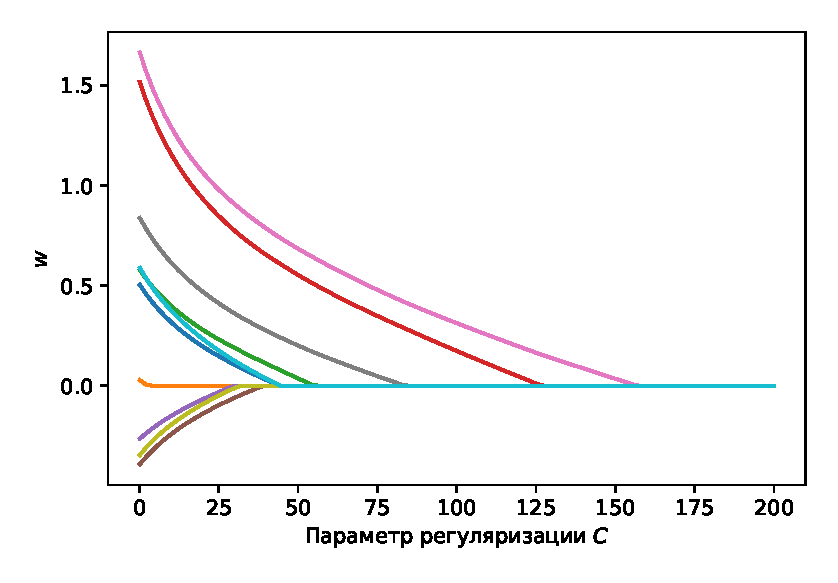
\includegraphics[width=0.5\textwidth]{../figures/log_reg_cs_exp.eps}
% 	\caption{Sample figure caption.}
% 	\label{fig:fig1}
% \end{figure}

% \subsection{Tables}
% See awesome Table~\ref{tab:table}.

% The documentation for \verb+booktabs+ (`Publication quality tables in LaTeX') is available from:
% \begin{center}
% 	\url{https://www.ctan.org/pkg/booktabs}
% \end{center}


% \begin{table}
% 	\caption{Sample table title}
% 	\centering
% 	\begin{tabular}{lll}
% 		\toprule
% 		\multicolumn{2}{c}{Part}                   \\
% 		\cmidrule(r){1-2}
% 		Name     & Description     & Size ($\mu$m) \\
% 		\midrule
% 		Dendrite & Input terminal  & $\sim$100     \\
% 		Axon     & Output terminal & $\sim$10      \\
% 		Soma     & Cell body       & up to $10^6$  \\
% 		\bottomrule
% 	\end{tabular}
% 	\label{tab:table}
% \end{table}

% \subsection{Lists}
% \begin{itemize}
% 	\item Lorem ipsum dolor sit amet
% 	\item consectetur adipiscing elit.
% 	\item Aliquam dignissim blandit est, in dictum tortor gravida eget. In ac rutrum magna.
% \end{itemize}


\bibliographystyle{unsrtnat}
\bibliography{references}

\end{document}
